\subsection{Multi-Probe LSH}
Traditional LSH schemes directly return the objects in the exactly collision buckets.
Multi-probe LSH~\cite{lv2007multi} tries to probe more buckets in one hash table to reduce the number of hash tables while maintains similar performance.
Formally speaking, multi-probe LSH probes a sequence of buckets which are from the collision bucket and a sequence of perturbations, as \cref{tbl:multi-probe-lsh} shows.
\begin{table}[hbt]
\centering
\caption{Difference between basic LSH and multi-probe LSH}
\begin{tabular}{|c|c|}
\hline
  \textbf{Scheme} & \textbf{Query}\\ \hline
  Basic& $g(q)=(h_1(q), h_2(q), ..., h_M(q))$ \\ \hline
  Multi-Probe& $g(q){+}\Delta^{(i)}, i{=}1,2,...,T$, $\Delta^{(i)}{=}(\delta_1^{(i)}, \delta_2^{(i)}, ..., \delta_M^{(i)})$ \\ \hline
\end{tabular}
\label{tbl:multi-probe-lsh}
\end{table}

Then we are going to introduce how the perturbation sequences are constructed.
\subsubsection{Step-Wise Probing Sequence}
Given the properties of LSH, similar objects are more likely in the close buckets.
This motivates the step-wise probing sequence, which firstly probes all 1-step perturbations, then all 2-step perturbations, and so on.
There are $L{\times} {M\choose n} {\times} 2^{n}$ n-step perturbations in total, where $L$ denotes the number of hash tables and $M$ denotes the number of compound hash functions in each table.

\subsubsection{Query-Based Probing Sequence}
Step-wise probing just consider all coordinates to be equally likely.
However, according the properties LSH, some perturbations are more likely than others.

We consider this hash function: $h(q)=\lfloor\frac{a\cdot q + b}{w}\rfloor$, where $w$ is a fixed hyper-parameter, $a$ is drawn from standard Gaussian, and $b$ is uniformly drawn from $[0, w)$.
For two objects $p, q$, $f(p) - f(q)$ follows Gaussian Distribution, where $f(q){=}a\cdot q {+} b$.
Therefore $P(h(p)=h(q)+\Delta)\approx C \exp(\sum_{i=1}^{M} x_i(\delta_i)^2)$, where $x_i(\delta_i)$ is the distance between q's projection and the boundary, like \cref{fig:x_i} shows.

\begin{figure}[hbt]
\centering
  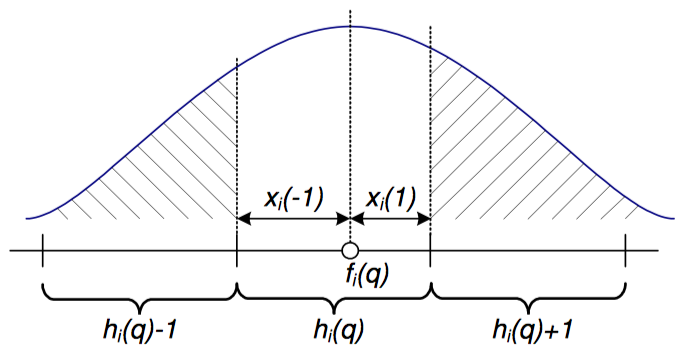
\includegraphics[width=\columnwidth]{figures/multi_probe_nn.png}
  \caption{$x_i(\delta)$}
  \label{fig:x_i}
\end{figure}

In order to find the probing sequence with smallest scores (defined as $score(\Delta)=\sum_{i=1}^{M}x_i(\delta_i)^2$), firstly we need to sort all $2M$ $x_i(\delta_i)$, then we use a heap to generate the probing sequence.

\subsubsection{Optimized Probing Sequence}

One of the drawback of query-based probing sequence is that it needs generating probing sequence for each query.
However, we can use an approximation to precompute it.
We denote the $j$-th elements in sorted $x_i(\delta_i)$ array  as $z_j$, then $z_j$ and $z_j^2$'s expectation is known and independent of query $q$.
Specifically speaking, $E[z_j]{=}\frac{j}{2(M+1)}W, E[z_j^2]{=}\frac{j(j+1)}{4(M+1)(M+2)}W^2$.
We use $\mathbb{E}[z_j^2]$ to replace $z_j^2$, then we only need to sort all $x_i(\delta_i)$ for each query.